\documentclass[tikz,border=3pt]{standalone}
\usepackage[utf8]{inputenc}
\usepackage[T1]{fontenc}
\usepackage{lmodern}
\renewcommand{\familydefault}{\sfdefault}
\usepackage{sansmath}\sansmath
\usepackage{chemfig}
\usepackage{pgfplots}\pgfplotsset{compat=1.18,/pgf/number format/use comma,/pgf/number format/1000 sep={.}}
\usetikzlibrary{arrows.meta,calc,positioning,decorations.pathmorphing,patterns}
% paleta del sitio
\definecolor{nar}{HTML}{E8680C}\definecolor{narc}{HTML}{FFB35C}\definecolor{hielo}{HTML}{FFF3E8}
\definecolor{tinta}{HTML}{1D1D1F}\definecolor{gris}{HTML}{6E6E73}\definecolor{lila}{HTML}{7C5CF0}
\definecolor{azul}{HTML}{2F6FD6}\definecolor{menta}{HTML}{17A673}\definecolor{coral}{HTML}{E8342A}
\begin{document}
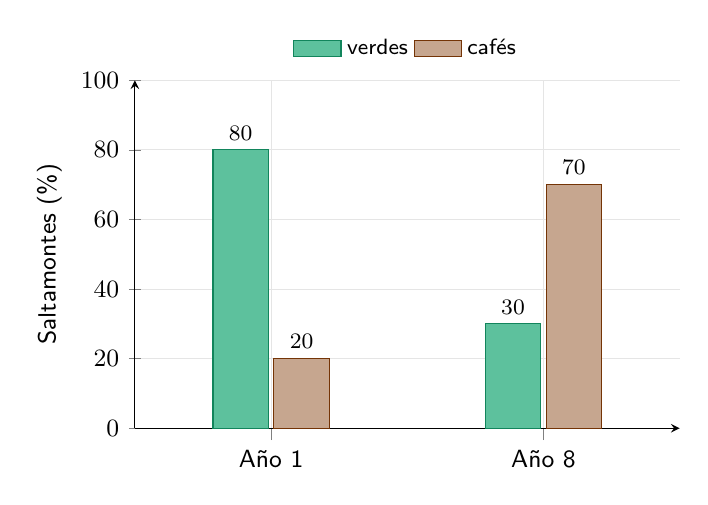
\begin{tikzpicture}[font=\small]
\begin{axis}[width=8.5cm,height=6cm,axis lines=left,ybar,area legend,bar width=20pt,
  ymin=0,ymax=100,ytick={0,20,...,100},grid=major,grid style={gray!20},
  symbolic x coords={Año 1,Año 8},xtick=data,enlarge x limits=0.5,
  ylabel={Saltamontes (\%)},nodes near coords,nodes near coords style={font=\footnotesize},
  legend style={at={(0.5,1.03)},anchor=south,legend columns=2,font=\footnotesize,draw=none}]
\addplot[fill=menta!70,draw=menta!80!black] coordinates {(Año 1,80) (Año 8,30)};
\addlegendentry{verdes}
\addplot[fill=nar!55!black!45,draw=nar!50!black] coordinates {(Año 1,20) (Año 8,70)};
\addlegendentry{cafés}
\end{axis}
\end{tikzpicture}
\end{document}
